
all of the models converged!!



\section{Analysis}

\subsection{What trends, correlations, and/or patterns do you see in the data?}

Different trends were observed for different data. This section will outline the results of our analysis for the three crops.

\subsubsection{Meat Chickens}

The data frame used for the final analysis contained eight observations.
When the prices and production were plotted using a scatterplot, a clear linear relationship was observed.
The scatterplot and trend-line for this relationship can be observed in Figure~\ref{fig:chicken_scatter}.
Using the statsmodels package in Python, we determined the coefficients for the linear model using the ordinary least squares (OLS) approach.
The output from the regression can be viewed in Figure~\ref{fig:chicken_ols}.

\begin{figure}
    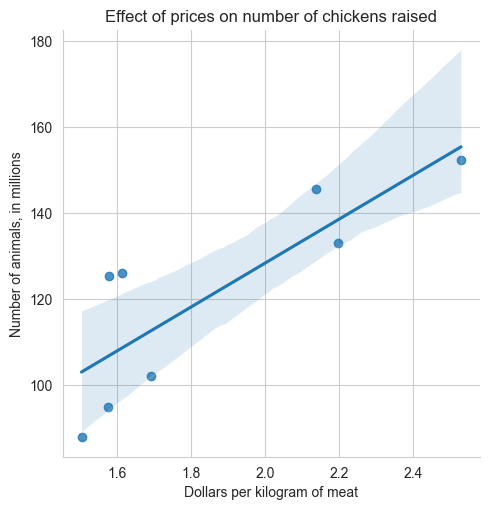
\includegraphics[width=\linewidth]{chicken_scatter}
    \caption{A scatter plot of Meat Chicken prices vs. Meat Chicken production.}
    \label{fig:chicken_scatter}
\end{figure}

The null hypothesis for this test was that no relationship exists between price and production.
Following the regression, there was the resulting model:

\\~\\

\tabto{5cm} $y = 26.4810 + 50.9459x_1$


\begin{itemize}
    \item Where $y$ is the number of chickens, measured in millions of individuals
    \item and $x_1$ is the price of chicken meat, in dollars per kilogram
\end{itemize}

\begin{figure}
    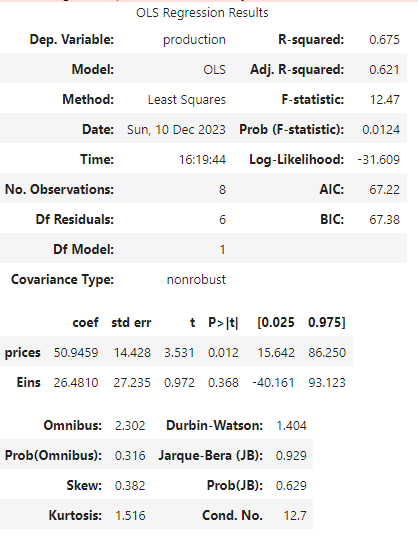
\includegraphics[width=\linewidth]{chicken_ols_results}
    \caption{Results from an Ordinary Least Squares Regression performed on Chickens raised in Canada.}
    \label{fig:chicken_ols}
\end{figure}

The F-statistic for this model was observed to be $12.47$; under a normal distribution the chances of observing this value are approximately $0.01\%$.
Setting our p-value to $0.05$, we would be forced to reject the null hypothesis and conclude there is indeed a relationship between the price and production of chicken in Canada.
Finally, The observed value for $R^2$ was $0.675$ which means that approximately 67\% of the variance of the data can be accounted for by this model.

\subsubsection{Hogs}

The data frame used for the final analysis contained a total of 38 observations.
When the prices and production were plotted using a scatterplot, the ellipsoid did not appear to have any meaningful structure.
The scatterplot and trend-line are displayed in Figure~\ref{fig:hog_scatter}.
Using the statsmodels package in Python, we determined the coefficients for the linear model using the ordinary least squares (OLS) approach.
The output from the regression can be viewed in Figure~\ref{fig:hog_ols}.

\begin{figure}
    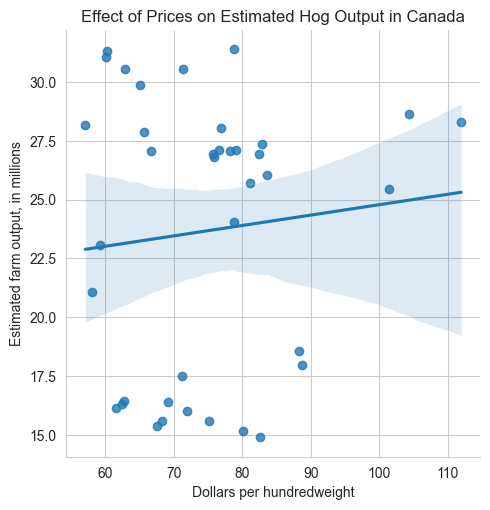
\includegraphics[width=\linewidth]{hog_scatter}
    \caption{A scatter plot of hog prices vs. hog production in Canada.}
    \label{fig:hog_scatter}
\end{figure}

The null hypothesis for this test was that no relationship exists between price and production.
Following the regression, there was the resulting model:

\\~\\

\tabto{5cm} $y = 20.3703 + 0.0441x_1$

\begin{itemize}
    \item Where $y$ is the estimated output of farms, measured in millions of individuals
    \item and $x_1$ is the price of hog, in dollars per hundredweight
\end{itemize}

\begin{figure}
    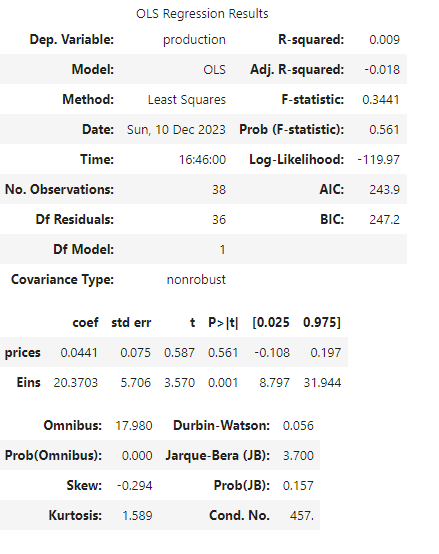
\includegraphics[width=\linewidth]{hog_ols_results}
    \caption{Results from an Ordinary Least Squares Regression performed on hog production in Canada.}
    \label{fig:hog_ols}
\end{figure}


The F-statistic for this model was observed to be $0.3441$.
With our p-value set to $0.05$, the null hypothesis that no relationship exists between the price and production of hogs in Canada would be accepted.
Based on the observed $R^2$ was $0.009$, we can state that effective none of the variance in the dataset was explained by this model.

\subsubsection{Wheat}

The data frame used for the final analysis contained 22 observations.
When the prices and production were plotted using a scatterplot, some degree of linearity was observed.
The scatterplot and trend-line for this relationship can be observed in Figure~\ref{fig:wheat_scatter}.
Using the statsmodels package in Python, we determined the coefficients for the linear model using the ordinary least squares (OLS) approach.
The output from the regression can be viewed in Figure~\ref{fig:wheat_ols}.

\begin{figure}
    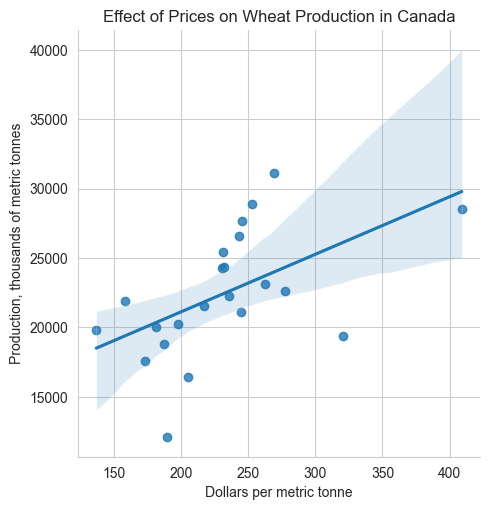
\includegraphics[width=\linewidth]{wheat_scatter}
    \caption{A scatter plot of wheat prices vs. wheat production.}
    \label{fig:wheat_scatter}
\end{figure}

The null hypothesis for this test was that no relationship exists between price and production.
Following the regression, there was the resulting model:

\\~\\

\tabto{5cm} $y = 1.285e4 + 41.3883x_1$

\begin{itemize}
    \item Where $y$ is the production of wheat, in thousands of metric tonnes
    \item and $x_1$ is the price of wheat, in dollars per metric tonne
\end{itemize}

\begin{figure}
    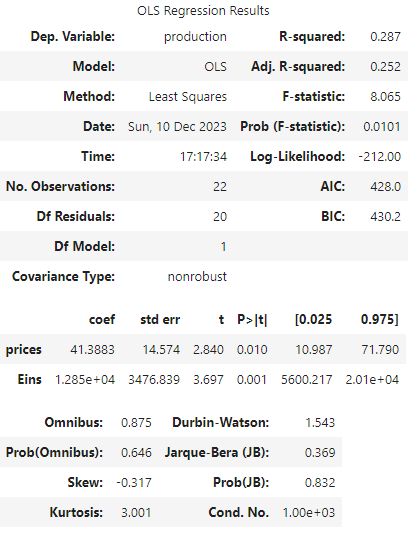
\includegraphics[width=\linewidth]{wheat_ols_results}
    \caption{Results from an Ordinary Least Squares Regression performed on wheat production in Canada.}
    \label{fig:wheat_ols}
\end{figure}

The F-statistic for this model was observed to be $8.065$; under a normal distribution the chances of observing this value are approximately $0.01\%$.
With a p-value set to $0.05$, we would be forced to reject the null hypothesis and conclude there is indeed a relationship between the price and production of wheat in Canada, albeit not as strong of a relationship as with chicken meat.
Finally, The observed value for $R^2$ was $0.287$ which means that approximately 29\% of the variance of the data can be accounted for by this model.
While this finding is significant, it is clear there are more factors involved in understanding the variations of production of wheat in Canada than solely price.


